\subsubsection{UC\theuccount-GP - Modifica utente}
		\begin{figure}[H]
			\centering
				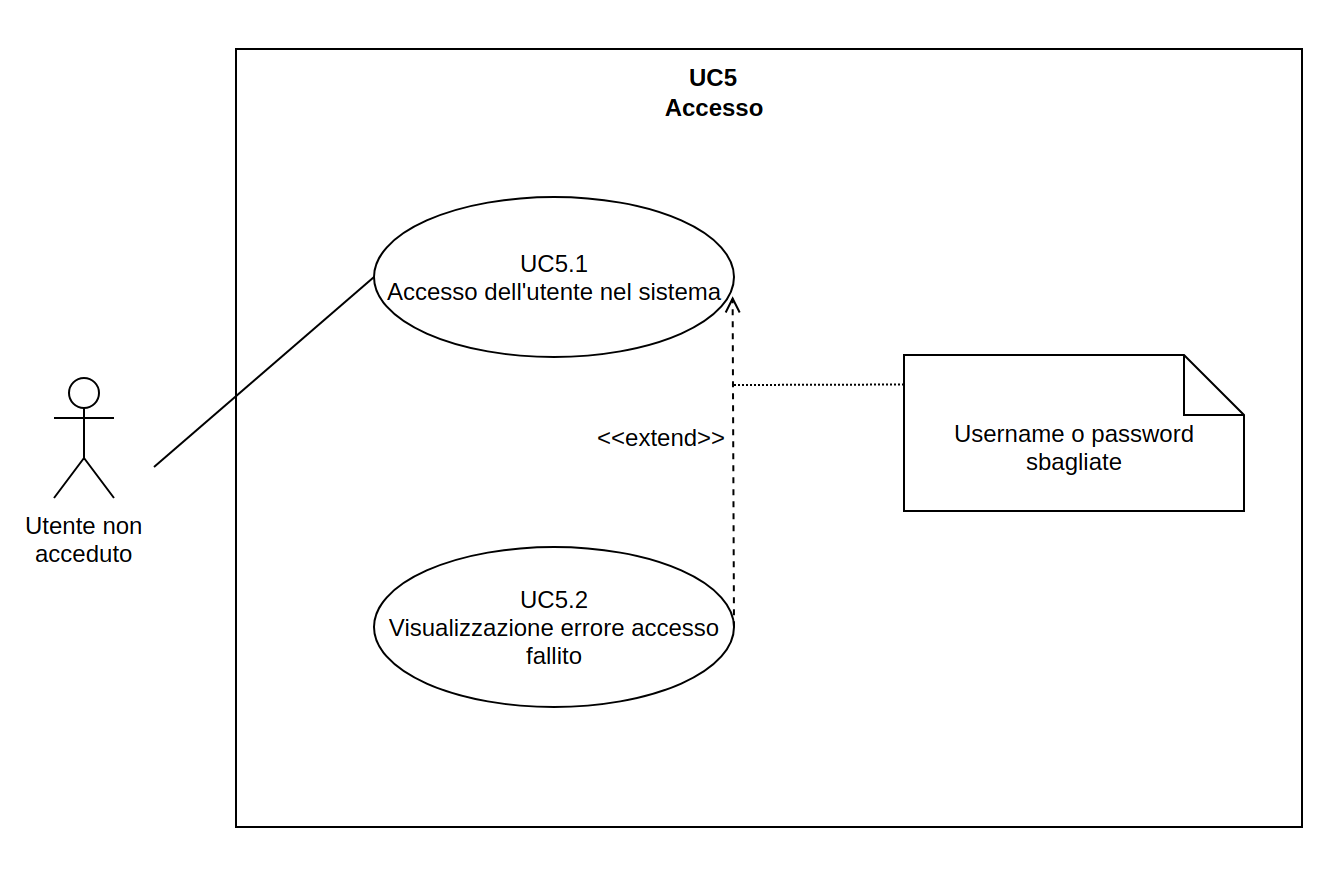
\includegraphics[width=\columnwidth]{img/UC5.png}\\
			\caption{UC\theuccount-GP - Modifica utente}
		\end{figure}
	\begin{itemize}
		\item \textbf{Codice}: UC\theuccount-GP.
		\item \textbf{Titolo}: modifica utente.
		\item \textbf{Attori primari}: utente acceduto.
		\item \textbf{Descrizione}: l’utente vuole modificare le informazioni relative a un utente.
		\item \textbf{Precondizione}: l'utente acceduto vuole modificare un utente già presente.
		\item \textbf{Postcondizione}: i campi dell'utente sono stati modificati correttamente.
		\item \textbf{Scenario Principale}:
		\begin{enumerate}
			\item Utente acceduto procede alla modifica di un utente.
		\end{enumerate}
	\end{itemize}

	\paragraph{UC\theuccount.1-GP - Selezione ID utente}
		\begin{figure}[H]
			\centering
			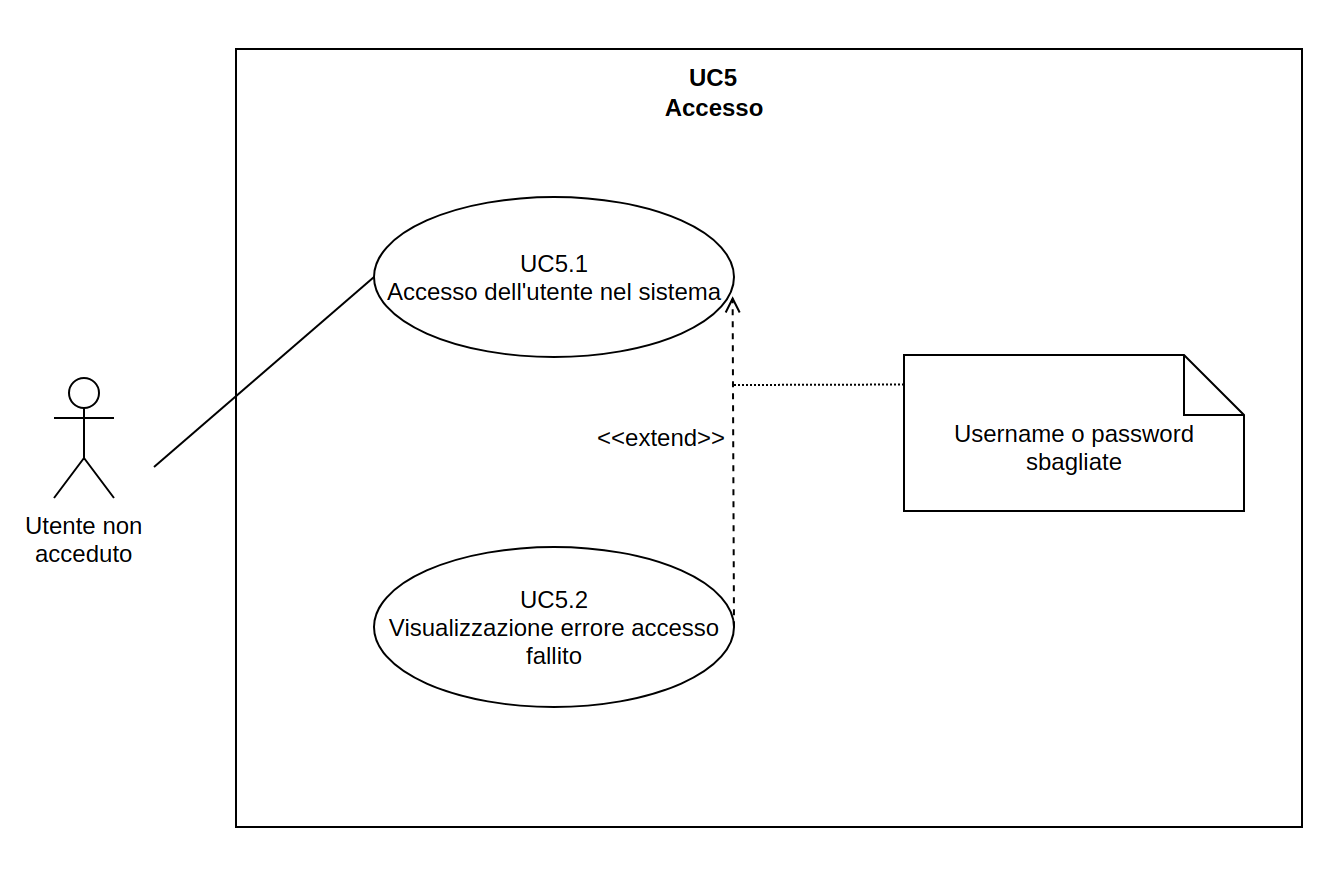
\includegraphics[width=\columnwidth]{img/UC5.png}\\
			\caption{UC\theuccount.1-GP - Selezione ID utente}
		\end{figure}
		\begin{itemize}
			\item \textbf{Codice}: UC\theuccount.1-GP.
			\item \textbf{Titolo}: selezione ID utente.
			\item \textbf{Attori primari}: utente acceduto.
			\item \textbf{Descrizione}: l'utente ha aggiunto il nuovo nome dell'utente che vuole modificare.
			\item \textbf{Precondizione}: l'utente acceduto vuole modificare un utente già presente.
			\item \textbf{Postcondizione}: l'ID utente è stato inserito.
			\item \textbf{Scenario Principale}:
			\begin{enumerate}
				\item Utente acceduto procede all'inserimento dell'ID utente da modificare.
			\end{enumerate}
			\item \textbf{Estensioni}:
			\begin{itemize}
				\item Errore user ID inesistente[UC15.2-GP]
			\end{itemize}
		\end{itemize}
	
		\subparagraph{UC\theuccount.1.1-GP - Modifica utente avvenuta con successo}
			\begin{figure}[H]
				\centering
				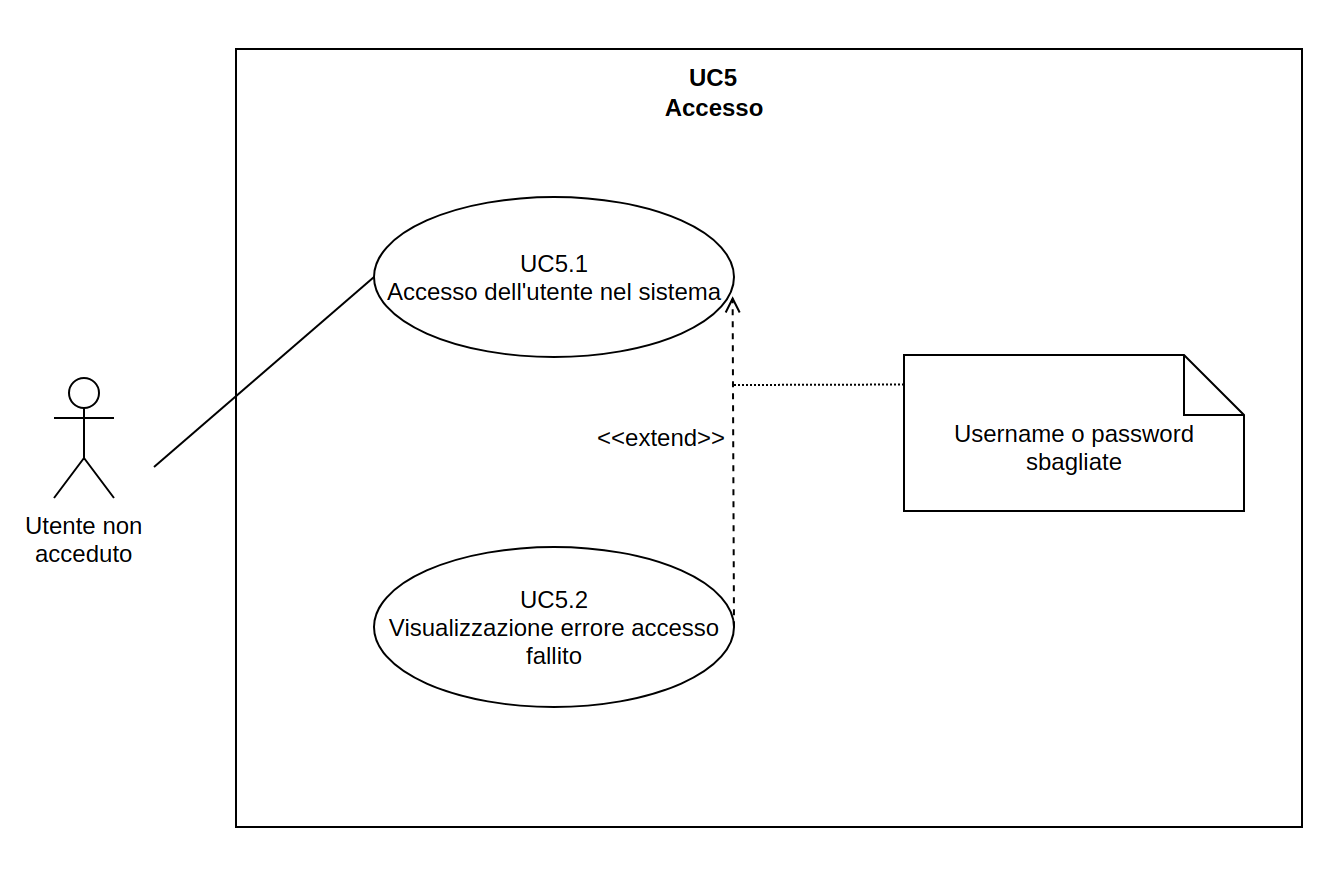
\includegraphics[width=\columnwidth]{img/UC5.png}\\
				\caption{UC\theuccount.1.1-GP - Modifica utente avvenuta con successo}
			\end{figure}
			\begin{itemize}
				\item \textbf{Codice}: UC\theuccount.1.1-GP.
				\item \textbf{Titolo}: modifica utente avvenuta con successo.
				\item \textbf{Attori primari}: utente acceduto.
				\item \textbf{Descrizione}: l'ID utente è presente nel sistema e ne vengono modificati i relativi campi con successo.
				\item \textbf{Precondizione}: l'utente acceduto vuole modificare un utente già presente.
				\item \textbf{Postcondizione}: l'utente è stato modificato con successo.
				\item \textbf{Scenario Principale}:
				\begin{enumerate}
					\item Utente viene modificato con successo.
				\end{enumerate}
			\end{itemize}
		
			\subsubparagraph{UC\theuccount.1.1.1-GP - Inserimento del nuovo nome}
				\begin{figure}[H]
					\centering
					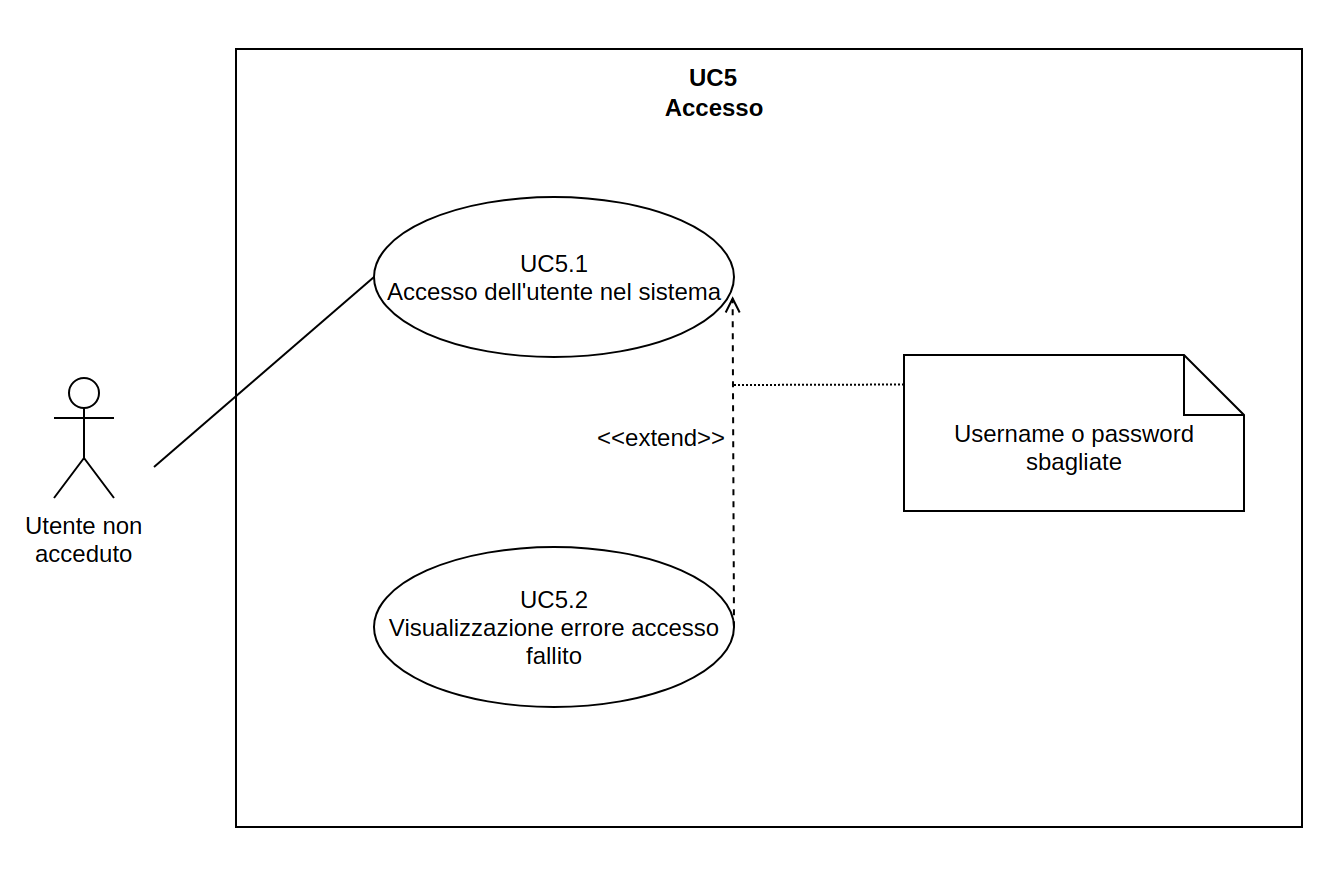
\includegraphics[width=\columnwidth]{img/UC5.png}\\
					\caption{UC\theuccount.1.1.1-GP - Inserimento del nuovo nome}
				\end{figure}
				\begin{itemize}
					\item \textbf{Codice}: UC\theuccount.1.1.1-GP.
					\item \textbf{Titolo}: inserimento del nuovo nome.
					\item \textbf{Attori primari}: utente acceduto.
					\item \textbf{Descrizione}: l'utente aggiunge il nuovo nome relativo all'ID utente inserito che vuole modificare.
					\item \textbf{Precondizione}: l'utente acceduto vuole modificare un utente già presente.
					\item \textbf{Postcondizione}: il nome è stato inserito.
					\item \textbf{Scenario Principale}:
					\begin{enumerate}
						\item Utente acceduto inserisce il nuovo nome dell'utente che vuole modificare.
					\end{enumerate}
				\end{itemize}
			
			\subsubparagraph{UC\theuccount.1.1.2-GP - Inserimento del nuovo cognome}
				\begin{figure}[H]
					\centering
					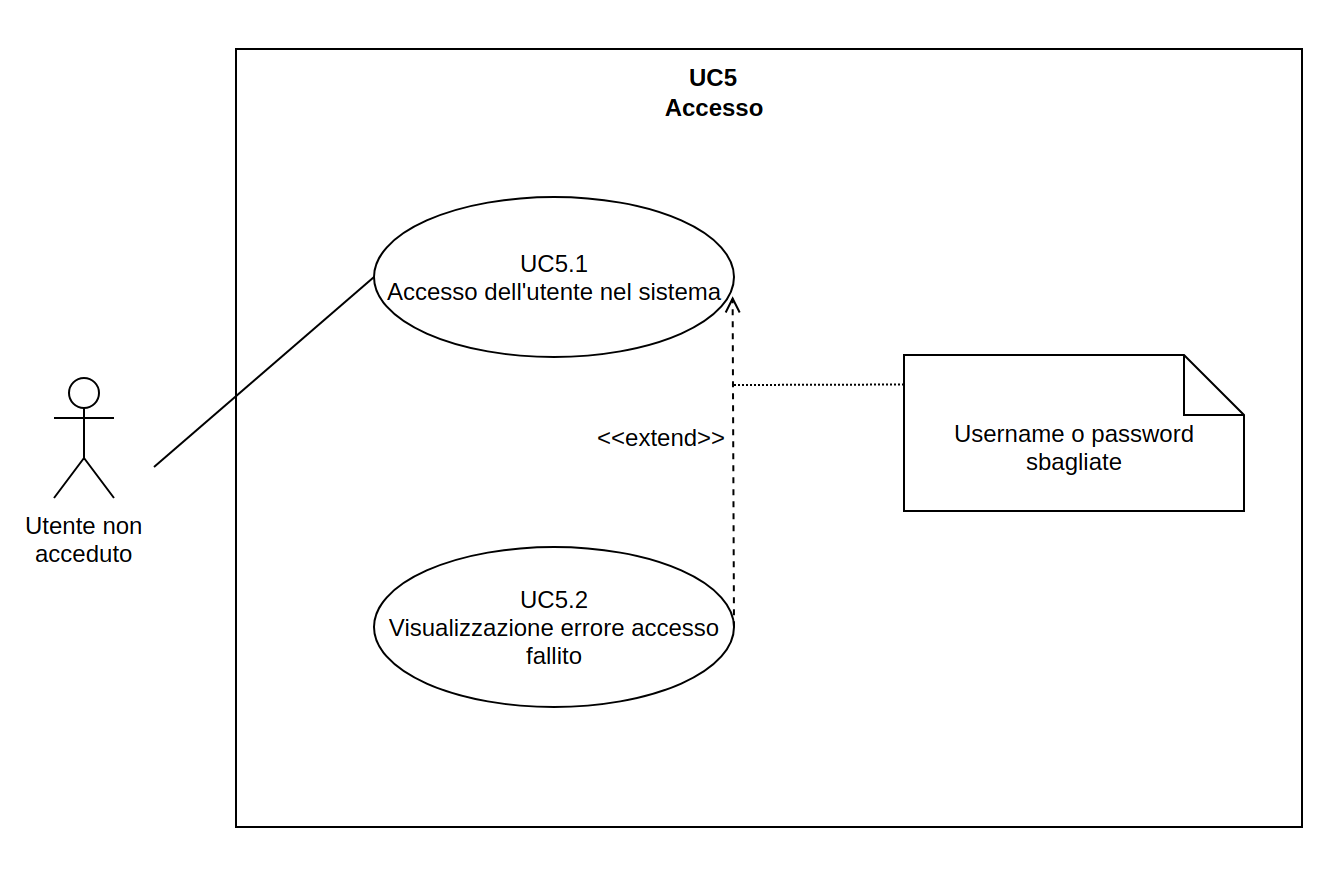
\includegraphics[width=\columnwidth]{img/UC5.png}\\
					\caption{UC\theuccount.1.1.2-GP - Inserimento del nuovo cognome}
				\end{figure}
				\begin{itemize}
					\item \textbf{Codice}: UC\theuccount.1.1.2-GP.
					\item \textbf{Titolo}: inserimento del nuovo cognome.
					\item \textbf{Attori primari}: utente acceduto.
					\item \textbf{Descrizione}: l'utente aggiunge il nuovo cognome relativo all'ID utente inserito che vuole modificare.
					\item \textbf{Precondizione}: l'utente acceduto vuole modificare un utente già presente.
					\item \textbf{Postcondizione}: il cognome è stato inserito.
					\item \textbf{Scenario Principale}:
					\begin{enumerate}
						\item Utente acceduto inserisce il nuovo cognome dell'utente che vuole modificare.
					\end{enumerate}
				\end{itemize}
			
			\subsubparagraph{UC\theuccount.1.1.3-GP - Inserimento del nuovo contatto Email}
				\begin{figure}[H]
					\centering
					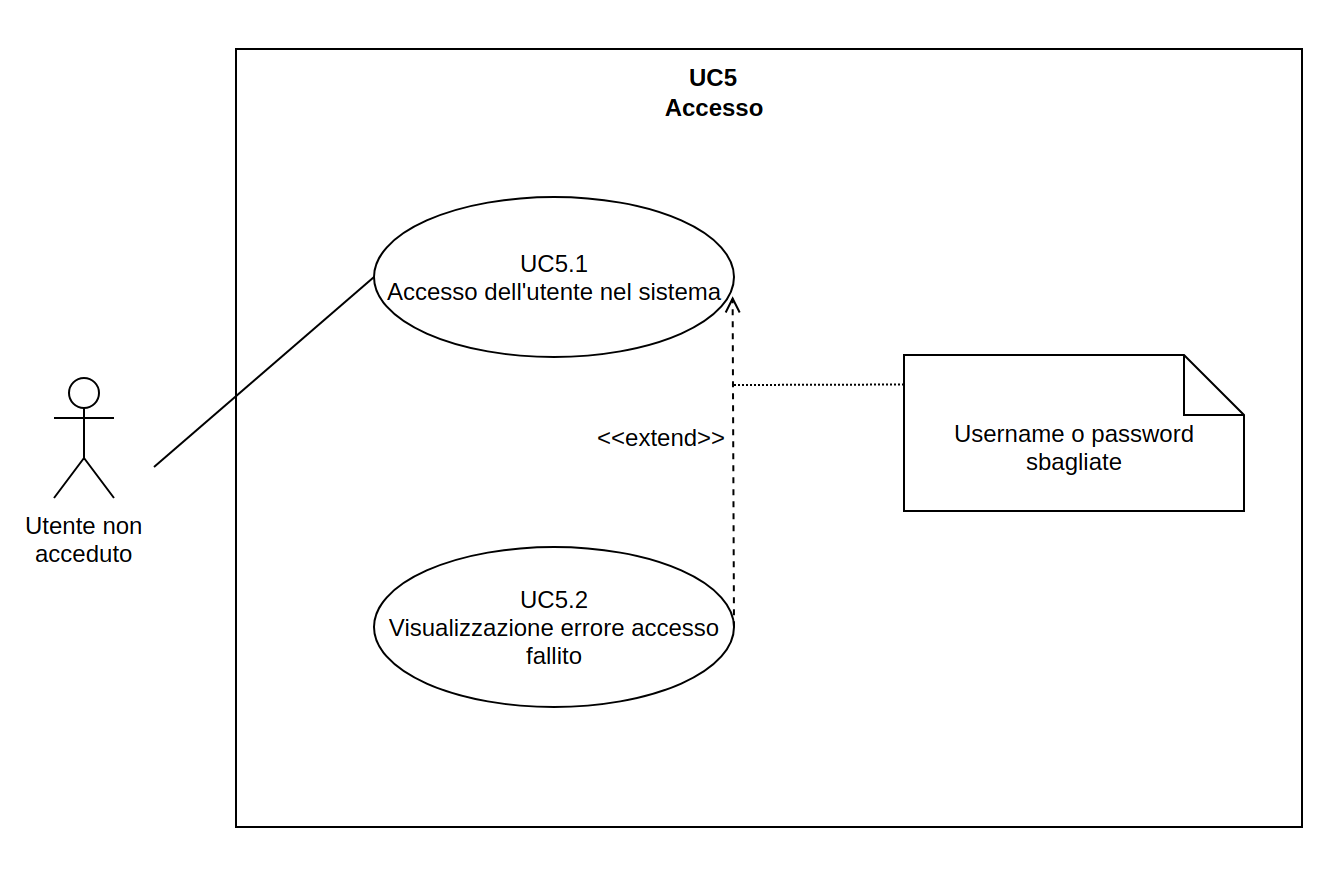
\includegraphics[width=\columnwidth]{img/UC5.png}\\
					\caption{UC\theuccount.1.1.3-GP - Inserimento del nuovo contatto Email}
				\end{figure}
				\begin{itemize}
					\item \textbf{Codice}: UC\theuccount.1.1.3-GP.
					\item \textbf{Titolo}: inserimento del nuovo contatto Email.
					\item \textbf{Attori primari}: utente acceduto.
					\item \textbf{Descrizione}: l'utente aggiunge il nuovo contatto Email relativo all'ID utente inserito che vuole modificare.
					\item \textbf{Precondizione}: l'utente acceduto vuole modificare un utente già presente.
					\item \textbf{Postcondizione}: il contatto Email è stato inserito.
					\item \textbf{Scenario Principale}:
					\begin{enumerate}
						\item Utente acceduto inserisce il nuovo contatto Email dell'utente che vuole modificare.
					\end{enumerate}
				\end{itemize}
			
			\subsubparagraph{UC\theuccount.1.1.4-GP - Inserimento del nuovo contatto Telegram}
				\begin{figure}[H]
					\centering
					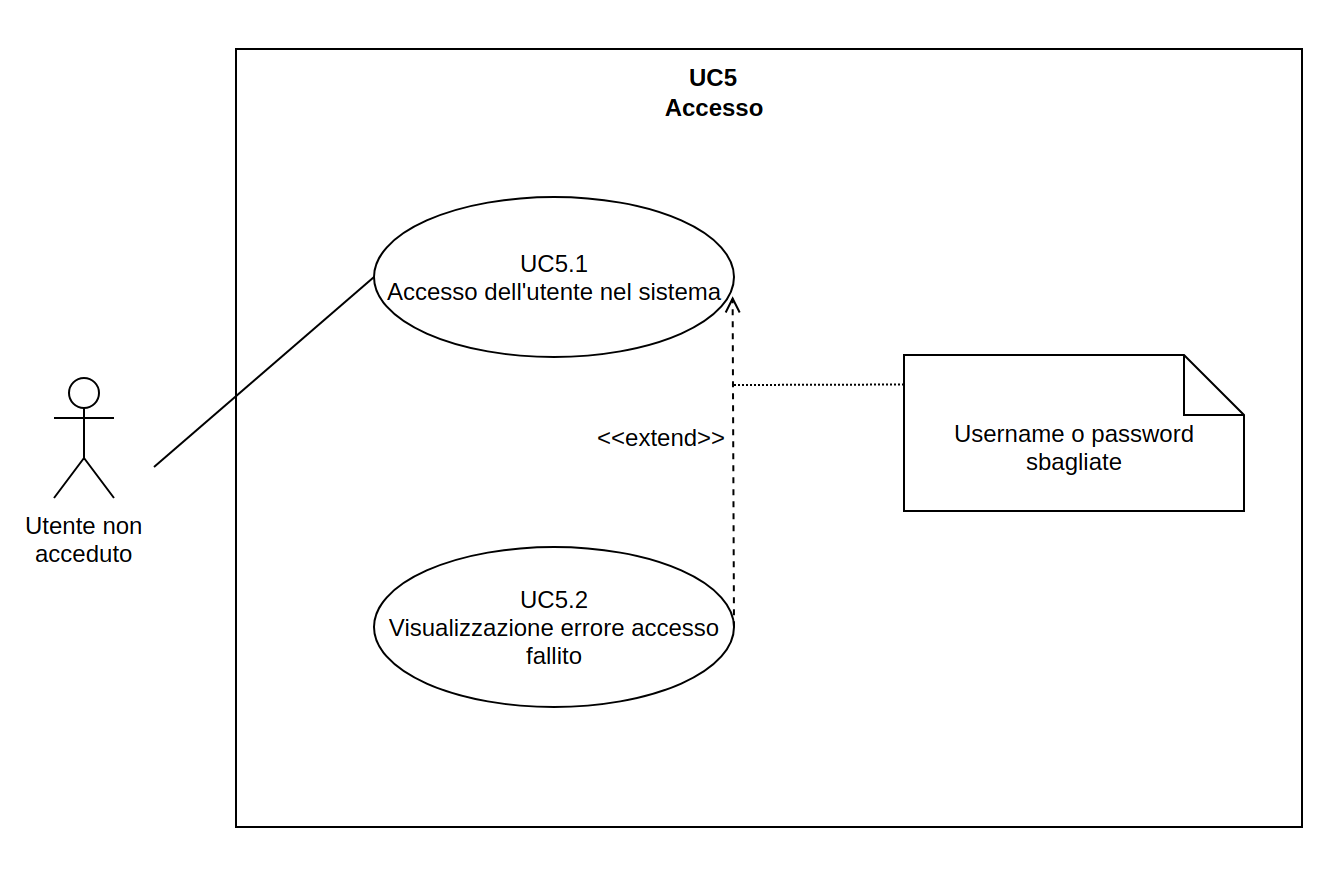
\includegraphics[width=\columnwidth]{img/UC5.png}\\
					\caption{UC\theuccount.1.1.4-GP - Inserimento del nuovo contatto Telegram}
				\end{figure}
				\begin{itemize}
					\item \textbf{Codice}: UC\theuccount.1.1.4-GP.
					\item \textbf{Titolo}: inserimento del nuovo contatto Telegram.
					\item \textbf{Attori primari}: utente acceduto.
					\item \textbf{Descrizione}: l'utente aggiunge il nuovo contatto Telegram relativo all'ID utente inserito che vuole modificare.
					\item \textbf{Precondizione}: l'utente acceduto vuole modificare un utente già presente.
					\item \textbf{Postcondizione}: il contatto Telegram è stato inserito.
					\item \textbf{Scenario Principale}:
					\begin{enumerate}
						\item Utente acceduto inserisce il nuovo contatto Telegram dell'utente che vuole modificare.
					\end{enumerate}
				\end{itemize}
		
	\paragraph{UC\theuccount.2-GP - Errore ID utente inesistente}
		\begin{figure}[H]
			\centering
			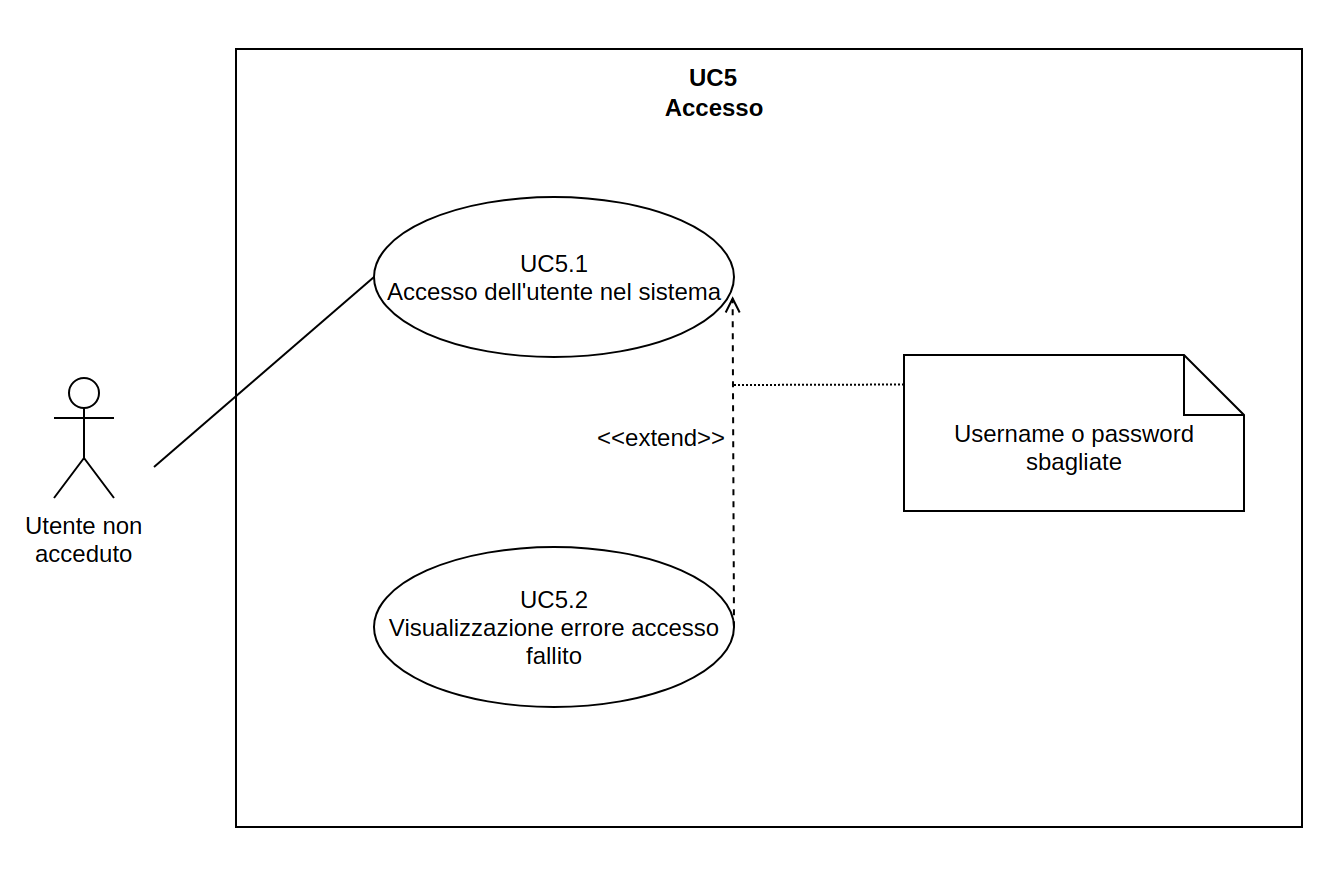
\includegraphics[width=\columnwidth]{img/UC5.png}\\
			\caption{UC\theuccount.2-GP - Errore ID utente inesistente}
		\end{figure}
		\begin{itemize}
			\item \textbf{Codice}: UC\theuccount.2-GP.
			\item \textbf{Titolo}: errore ID utente inesistente.
			\item \textbf{Attori primari}: utente acceduto.
			\item \textbf{Descrizione}:  l’utente viene avvisato che ha inserito un'ID utente errato.
			\item \textbf{Precondizione}: l'utente acceduto vuole modificare un utente già presente.
			\item \textbf{Postcondizione}: il sistema comunica all’utilizzatore l’errore.
			\item \textbf{Scenario Principale}:
			\begin{enumerate}
				\item L'utente ha inserito un ID utente errato e il sistema comunica all’utilizzatore l’errore.
			\end{enumerate}
		\end{itemize}